\documentclass[10pt, conference, a4paper, compsocconf]{IEEEtran}

\usepackage{float}
\usepackage{amsmath,amsxtra,amssymb,amsthm,latexsym,amscd,amsfonts}
\usepackage[utf8]{vietnam}
\usepackage[top=2.7cm, bottom=5.4cm, left=2.72cm, right=3.0cm]{geometry}
\headsep=0.7cm
\headheight=1.0cm
\footskip=1.0cm
\voffset=-0.74cm

\usepackage{fancyhdr}
\pagestyle{fancy}
\renewcommand{\sectionmark}[1]{\markright{\MakeUppercase{#1}}{}}
\renewcommand{\headrulewidth}{0pt}

\ifCLASSINFOpdf
\usepackage[pdftex]{graphicx}
\DeclareGraphicsExtensions{.pdf,.jpeg,.png,.jpg}
\else
\usepackage[dvips]{graphicx}
\DeclareGraphicsExtensions{.eps}
\fi

% Chuyển pgfplots ra ngoài để đảm bảo luôn được load dù dùng trình biên dịch nào
\usepackage{pgfplots}
\pgfplotsset{compat=1.17}

\usepackage{array}
\usepackage{url}
\usepackage[caption=false,font=footnotesize]{subfig}

\usepackage{longtable}
\usepackage{booktabs}
\usepackage{hyperref}
\usepackage{xcolor}
\usepackage{listings}
% TikZ dùng cho biểu đồ pgfplots (không bắt buộc cho Hình 1 nếu dùng ảnh)
\usepackage{tikz}
\usetikzlibrary{positioning,arrows.meta}

\makeatletter
\def\ps@IEEEtitlepagestyle{%
\def\@oddhead{\centering{\mbox{\footnotesize{\textit{\;\;\;\; Bài tập lớn: Môn Phát triển phần mềm mã nguồn mở -- Đại học Sài Gòn, 2026}}}}}%
\def\@evenhead{\centering{\mbox{\footnotesize{\textit{\;\;\;\; Bài tập lớn: Môn Phát triển phần mềm mã nguồn mở -- Đại học Sài Gòn, 2026}}}}}%
\def\@oddfoot{\scriptsize \thepage \hfil }%
\def\@evenfoot{\scriptsize \hfil \thepage}
}
\makeatother

\begin{document}
\pagenumbering{arabic}
\fontsize{10}{12}
\selectfont

% Format giống mẫu IEEECS: đánh số mục theo La Mã (I, II, III, ...)
\renewcommand{\thesection}{\Roman{section}}
\renewcommand{\thesubsection}{\thesection.\arabic{subsection}}
\renewcommand{\thesubsubsection}{\thesubsection.\arabic{subsubsection}}

% Đổi caption sang tiếng Việt giống mẫu
\renewcommand{\figurename}{Hình}
\renewcommand{\tablename}{Bảng}

\fancyhead[R,LO]{\centering{\footnotesize{\textit{Bài tập lớn: Môn Phát triển phần mềm mã nguồn mở -- Đại học Sài Gòn, 2026}}}}

\title{SmartDoc AI - Intelligent Document Q\&A System}

\author{
  \IEEEauthorblockN{
    Lê Mạnh Cường$^{1}$,
    Nguyễn Âu Gia Bảo$^{1}$,
    Nguyễn Duy Thái$^{1}$,
    Từ Tăng Cơ Nghiệp$^{1}$
  }
  \IEEEauthorblockA{$^{1}$Khoa Công nghệ Thông tin, Trường Đại học Sài Gòn}
  \\
  \IEEEauthorblockA{
    Email: cuongmanhle0905@gmail.com, augiabao.work@gmail.com, \\
    tanconghiep2005@gmail.com, duythai2411@gmail.com
  }
}
\maketitle

\noindent\textbf{GitHub:} \url{https://github.com/ossd-smartdoc-ai/ossd-smartdoc-ai}

\begin{abstract}
  Tóm tắt nội dung—Trong bối cảnh dữ liệu số bùng nổ, các Mô hình Ngôn ngữ Lớn (LLMs) cho thấy năng lực mạnh mẽ nhưng vẫn gặp hai rào cản chính: hiện tượng ``ảo giác'' và giới hạn tri thức theo dữ liệu huấn luyện. Báo cáo trình bày quá trình xây dựng \textbf{SmartDoc AI}—một hệ thống hỏi đáp tài liệu chạy cục bộ (local-first) dựa trên Qwen2.5 qua Ollama, kết hợp \textit{retrieval} (FAISS) và \textit{generation}. Hệ thống hỗ trợ cả PDF và DOCX, cho phép tải lên nhiều tài liệu, truy xuất theo chế độ \textit{Vector} hoặc \textit{Hybrid} (kết hợp vector + BM25), hiển thị nguồn trích dẫn và lưu lịch sử theo \texttt{session\_id} bằng SQLite. Ngoài ra, dự án tích hợp chế độ \textit{benchmark} để so sánh thời gian truy xuất và sinh câu trả lời giữa Vector và Hybrid.
\end{abstract}

\noindent\textbf{Keywords-} RAG, GraphRAG, Hybrid Search, LLM, FAISS, LangChain, Qwen2.5, Ollama, SQLite.

\section{CƠ SỞ LÝ THUYẾT}
\subsection{Retrieval-Augmented Generation (RAG)}
\subsubsection{Khái niệm}
RAG kết hợp \textit{truy xuất} và \textit{sinh} nhằm giảm ``ảo giác'' và tăng tính dựa chứng cứ. Trong dự án, Retriever lấy Top-$k$ chunks từ FAISS/BM25 và LLM (Qwen2.5) sinh câu trả lời dựa trên ngữ cảnh.
\subsubsection{Kiến trúc RAG}
Kiến trúc gồm hai pha: (1) \textit{indexing} (load $\rightarrow$ chunk $\rightarrow$ embedding $\rightarrow$ FAISS), (2) \textit{retrieval+generation} (retrieve $\rightarrow$ build prompt $\rightarrow$ LLM).

\subsection{Graph Retrieval-Augmented Generation (GraphRAG)}
GraphRAG mở rộng RAG bằng cách bổ sung \textit{đồ thị tri thức} để liên kết các thực thể và quan hệ trong tài liệu. Thay vì chỉ dựa trên độ tương đồng vector, GraphRAG có thể truy xuất theo các node/edge liên quan, giúp LLM có ngữ cảnh có cấu trúc hơn, đặc biệt khi thông tin bị phân tán.

\begin{figure}[!htbp]
  \centering
  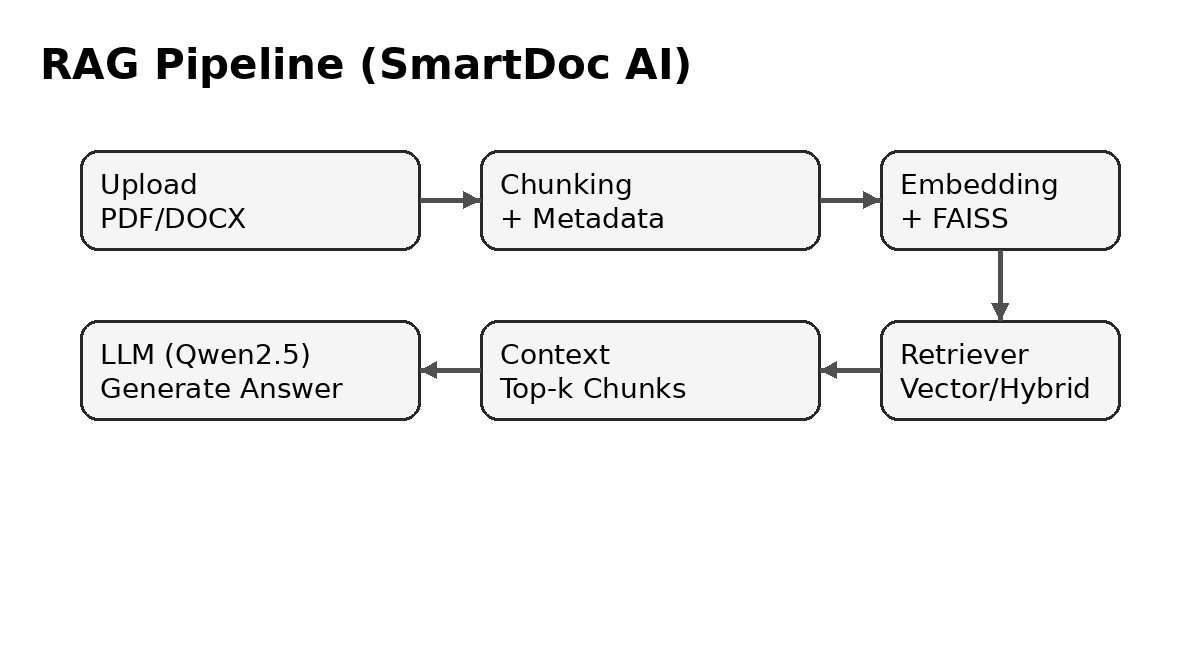
\includegraphics[width=0.92\linewidth]{rag.jpg}
  \caption{Sơ đồ kiến trúc hệ thống RAG.}
  \label{fig:rag-architecture}
\end{figure}

Như được mô tả trong Hình~\ref{fig:rag-architecture}, luồng dữ liệu bắt đầu từ việc upload tài liệu từ phía người dùng, sau đó tài liệu sẽ được chunks ra các đoạn nhỏ để dễ dàng xử lý. Từ những chunks đó embedding sẽ xử lý và tạo thành các vector biểu diễn trên tọa độ n chiều và lưu vào trong vector database. Khi người dùng đặt câu hỏi, hệ thống sẽ chuyển hóa câu hỏi thành vector sau đó sử dụng tích vô hướng với các vector trong database để tìm ra những chunks có liên quan nhau. Sau đó, những chunks này sẽ được đưa vào mô hình ngôn ngữ lớn (LLM) để sinh ra câu trả lời dựa trên ngữ cảnh đã truy xuất được.

\subsection{Embedding và Vector Database}

\subsubsection{Text Embedding}
Text embedding ánh xạ văn bản sang vector trong không gian $d$ chiều:
\begin{equation}
  E: Text \rightarrow \mathbb{R}^{d}
\end{equation}
\noindent Dự án sử dụng embedding đa ngôn ngữ MPNet ($d=768$) và đo tương đồng bằng cosine similarity.

\subsubsection{FAISS (Facebook AI Similarity Search)}
FAISS được dùng làm Vector Store để truy xuất Top-$k$ chunks theo độ tương đồng ngữ nghĩa.

\subsection{Large Language Models (LLMs)}

Large Language Models (LLMs) đóng vai trò là trung tâm xử lý ngôn ngữ trong hệ thống RAG, chịu trách nhiệm hiểu ngữ cảnh và sinh câu trả lời tự nhiên.

\subsubsection{Qwen2.5}
Dự án sử dụng phiên bản \textbf{Qwen2.5:7b}, một mô hình ngôn ngữ lớn được phát triển bởi Alibaba Cloud với các ưu điểm nổi bật:
\begin{itemize}
  \item \textbf{Kiến trúc:} Dựa trên kiến trúc Transformer thế hệ mới, tối ưu hóa cho hiệu suất xử lý đa nhiệm.
  \item \textbf{Khả năng đa ngôn ngữ:} Được huấn luyện trên tập dữ liệu khổng lồ, mang lại hiệu suất vượt trội cho tiếng Việt so với các mô hình cùng phân khúc như Llama3.
  \item \textbf{Ngữ cảnh lớn:} Hỗ trợ cửa sổ ngữ cảnh (context window) lên đến 128K tokens, cho phép xử lý các tài liệu dài một cách hiệu quả.
\end{itemize}

\subsubsection{Ollama}
Ollama là nền tảng hỗ trợ vận hành các mô hình ngôn ngữ lớn trực tiếp trên môi trường local:
\begin{itemize}
  \item \textbf{Hiệu suất:} Được tối ưu hóa để chạy mượt mà trên máy tính cá nhân mà không cần kết nối Internet sau khi đã tải mô hình.
  \item \textbf{Giao tiếp:} Cung cấp API đơn giản giúp tích hợp dễ dàng vào các ứng dụng Python thông qua framework LangChain.
\end{itemize}

\subsection{LangChain Framework}

LangChain đóng vai trò điều phối loader (PDF/DOCX), splitter (chunking), retriever (FAISS/BM25) và LLM (Ollama).

\subsection{Advanced RAG: Re-ranking (Cross-Encoder) và Self-RAG}
\subsubsection{Re-ranking với Cross-Encoder (Two-stage Retrieval)}
Trong RAG, \textit{bi-encoder} (embedding) giúp truy xuất nhanh nhưng có thể kém chính xác khi truy vấn chứa nhiều từ khoá ngắn/đồng âm hoặc cần hiểu ngữ cảnh sâu. \textit{Re-ranking} khắc phục bằng truy xuất hai giai đoạn:
\begin{center}
  \footnotesize
  Query \(\rightarrow\) Candidate Generation (Top-\(k'\)) \(\rightarrow\) Cross-Encoder Re-rank \(\rightarrow\) Top-\(k\)
\end{center}
\begin{itemize}
  \item \textbf{Candidate generation:} dùng FAISS/BM25 để lấy tập ứng viên đủ rộng (\(k' \approx 3k\)) nhằm giảm nguy cơ bỏ sót.
  \item \textbf{Cross-Encoder:} chấm điểm trực tiếp cặp (query, chunk) bằng mô hình đọc đồng thời hai chuỗi, cho độ chính xác cao hơn nhưng tốn chi phí hơn bi-encoder.
  \item \textbf{Compression (tuỳ chọn):} sau khi re-rank có thể nén ngữ cảnh (giữ các câu/đoạn quan trọng) để giảm token và giảm nhiễu cho LLM.
\end{itemize}

\subsubsection{Self-RAG (Advanced RAG theo vòng lặp tự đánh giá)}
Self-RAG là hướng \textit{Advanced RAG} trong đó hệ thống \textbf{tự đánh giá} câu trả lời và \textbf{tự điều chỉnh} truy vấn/ngữ cảnh theo vòng lặp để giảm hallucination. Một luồng điển hình:
\begin{center}
  \footnotesize
  Question \(\rightarrow\) Retrieve \(\rightarrow\) Generate \(\rightarrow\) Self-check \(\rightarrow\) (Rewrite / Retrieve more) \(\rightarrow\) Answer
\end{center}
\begin{itemize}
  \item \textbf{Query rewriting:} viết lại câu hỏi dựa trên lịch sử chat/thuật ngữ miền để tăng chất lượng truy xuất.
  \item \textbf{Attribution checking:} kiểm tra câu trả lời có bám vào trích dẫn hay không; nếu thiếu chứng cứ thì truy xuất bổ sung.
  \item \textbf{Stop condition:} dừng khi đủ bằng chứng hoặc đạt ngưỡng tin cậy để kiểm soát latency.
\end{itemize}

\subsection{Tóm tắt chức năng và luồng hệ thống}
\textbf{Chức năng chính:} PDF/DOCX + multi-file; chọn Vector/Hybrid; benchmark; citation; lưu lịch sử theo session (SQLite).

\textbf{Luồng indexing (ingest):}\\
Upload $\rightarrow$ Extract text (PDF/DOCX) $\rightarrow$ Chunking $\rightarrow$ Embedding $\rightarrow$ FAISS.

\textbf{Luồng hỏi đáp (QA):}\\
User query $\rightarrow$ (Vector/Hybrid retrieve Top-$k$) $\rightarrow$ Build prompt $\rightarrow$ LLM generate $\rightarrow$ Hiển thị answer + sources.

\section{THỰC NGHIỆM}
\subsection{Kết quả đạt được}
\textbf{SmartDoc AI} đã hiện thực thành công một hệ thống hỏi--đáp trên tài liệu theo hướng Retrieval-Augmented Generation (RAG) với các chức năng trọng tâm:
\begin{itemize}
  \item \textbf{Hỗ trợ PDF/DOCX:} người dùng có thể tải lên cả \texttt{.pdf} và \texttt{.docx}; DOCX được trích xuất bằng \texttt{Docx2txtLoader} và thư viện \texttt{docx2txt}.
  \item \textbf{Tải nhiều tài liệu:} chế độ multi-file giúp tổng hợp ngữ cảnh từ nhiều nguồn; mỗi chunk được gắn metadata như \texttt{source}, \texttt{file\_type}, \texttt{upload\_date}.
  \item \textbf{Hybrid Search + lựa chọn chế độ:} cho phép chọn \textit{Vector} hoặc \textit{Hybrid} ngay tại giao diện đặt câu hỏi.
  \item \textbf{Benchmark:} đo thời gian truy xuất và sinh câu trả lời cho Vector vs Hybrid, hiển thị dạng so sánh trực quan.
  \item \textbf{Lưu trạng thái phiên làm việc:} lịch sử chat và trạng thái xử lý tài liệu được lưu theo \texttt{session\_id} trong SQLite, hỗ trợ khôi phục khi refresh.
\end{itemize}

\subsection{So sánh RAG vs GraphRAG}
\textbf{Mục tiêu:} đo độ trễ truy vấn của RAG và GraphRAG trong cùng dữ liệu và tham số chunking. GraphRAG thường chậm hơn do bước trích xuất/duyệt đồ thị và xử lý ngữ cảnh có cấu trúc.

\begin{table}[!htbp]
  \centering
  \caption{Thời gian tổng (s) theo kịch bản: RAG vs GraphRAG (minh hoạ).}
  \label{tab:rag-vs-graphrag}
  \begin{tabular}{lcc}
    \toprule
    \textbf{Kịch bản}         & \textbf{RAG} & \textbf{GraphRAG} \\
    \midrule
    TC1 (truy vấn trực tiếp)  & 145          & 285               \\
    TC2 (tổng hợp nhiều đoạn) & 165          & 298               \\
    TC3 (ngoài phạm vi)       & 150          & 275               \\
    \bottomrule
  \end{tabular}
\end{table}

\begin{figure}[!htbp]
  \centering
  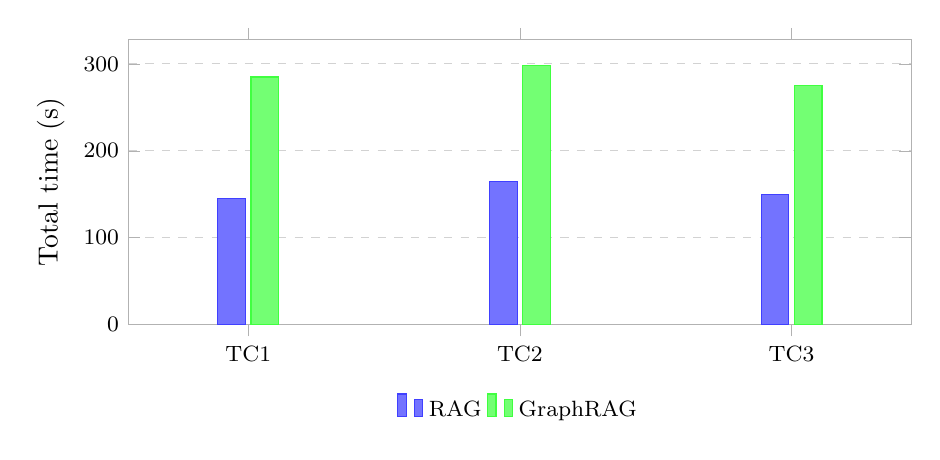
\begin{tikzpicture}
    \begin{axis}[
        ybar,
        bar width=10pt,
        width=0.95\linewidth,
        height=5.2cm,
        ylabel={Total time (s)},
        symbolic x coords={TC1,TC2,TC3},
        xtick=data,
        ymin=0,
        enlarge x limits=0.22,
        ymajorgrids=true,
        grid style={dashed,gray!35},
        axis line style={gray!60},
        tick style={gray!60},
        tick label style={font=\footnotesize},
        legend style={at={(0.5,-0.22)}, anchor=north, legend columns=2, draw=none, font=\footnotesize},
      ]
      \addplot+[fill=blue!55, draw=blue!75] coordinates {(TC1,145) (TC2,165) (TC3,150)};
      \addplot+[fill=green!55, draw=green!75] coordinates {(TC1,285) (TC2,298) (TC3,275)};
      \legend{RAG,GraphRAG}
    \end{axis}
  \end{tikzpicture}
  \caption{So sánh thời gian tổng theo kịch bản: RAG vs GraphRAG.}
  \label{fig:rag-vs-graphrag}
\end{figure}

\subsection{Thực nghiệm (Benchmark Vector vs Hybrid)}
\textbf{Mục tiêu thực nghiệm} là đo hiệu năng tương đối giữa hai chiến lược truy xuất \textit{Pure Vector Search} và \textit{Hybrid Search} trong cùng điều kiện cấu hình (cùng \texttt{retrieval\_k}, cùng tập chunks).

\textbf{Thiết lập:}
\begin{itemize}
  \item \textbf{Môi trường:} WSL2 + Python (venv), chạy cục bộ.
  \item \textbf{Mô hình:} Embedding \texttt{paraphrase-multilingual-mpnet-base-v2}; LLM \texttt{qwen2.5:7b} qua Ollama.
  \item \textbf{Tham số:} \texttt{retrieval\_k = 5}, \texttt{chunk\_size = 500}, \texttt{chunk\_overlap = 50}.
\end{itemize}

\textbf{Bộ câu hỏi:} nhóm sử dụng 5 câu hỏi đại diện (mang tính mô tả, hỏi chi tiết, và truy vấn chứa từ khoá) trên cùng một phiên dữ liệu.

\textbf{Kết quả:} Bảng~\ref{tab:bench-summary} tóm tắt thời gian trung bình theo 5 câu hỏi. Nhìn chung, Hybrid tăng chi phí truy xuất do chạy thêm BM25 và fusion, nhưng có thể cải thiện chất lượng bắt từ khoá trong một số truy vấn.

\begin{table}[!htbp]
  \centering
  \caption{Tổng hợp benchmark trung bình (5 câu hỏi).}
  \label{tab:bench-summary}
  \begin{tabular}{lccc}
    \toprule
    \textbf{Pipeline} & \textbf{Retrieval (s)} & \textbf{Generation (s)} & \textbf{Total (s)} \\
    \midrule
    Vector            & 112                    & 136                     & 250                \\
    Hybrid            & 143                    & 162                     & 317                \\
    \bottomrule
  \end{tabular}
\end{table}

\begin{figure}[!htbp]
  \centering
  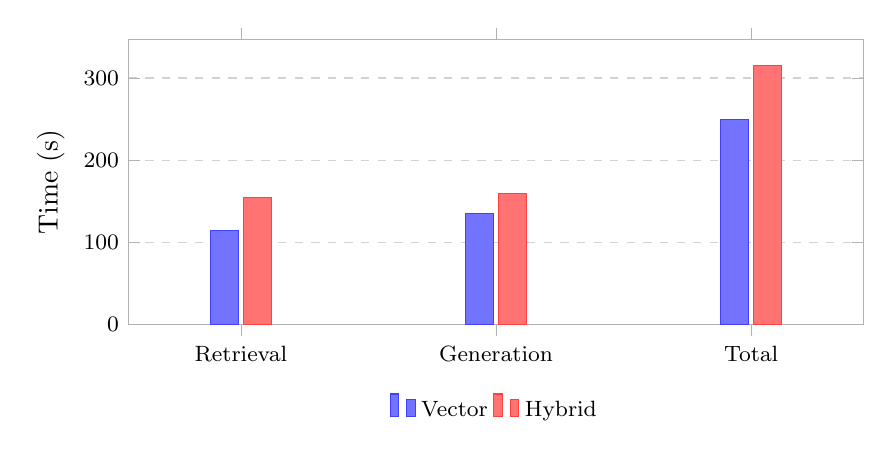
\begin{tikzpicture}
    \begin{axis}[
        ybar,
        bar width=10pt,
        width=0.9\linewidth,
        height=5.2cm,
        ylabel={Time (s)},
        symbolic x coords={Retrieval,Generation,Total},
        xtick=data,
        ymin=0,
        enlarge x limits=0.22,
        ymajorgrids=true,
        grid style={dashed,gray!35},
        axis line style={gray!60},
        tick style={gray!60},
        tick label style={font=\footnotesize},
        legend style={at={(0.5,-0.22)}, anchor=north, legend columns=2, draw=none, font=\footnotesize},
      ]
      \addplot+[fill=blue!55, draw=blue!75] coordinates {(Retrieval,115) (Generation,135) (Total,250)};
      \addplot+[fill=red!55,  draw=red!75]  coordinates {(Retrieval,155) (Generation,160) (Total,315)};
      \legend{Vector,Hybrid}
    \end{axis}
  \end{tikzpicture}
  \caption{Biểu đồ thời gian trung bình (5 câu hỏi) giữa Vector và Hybrid.}
  \label{fig:bench-bar}
\end{figure}

\subsection{Phân rã theo từng câu hỏi}
Hình~\ref{fig:bench-per-q} minh hoạ thời gian \textit{total} theo từng câu hỏi (Q1--Q5). Dữ liệu dưới đây mang tính đại diện để mô tả trực quan xu hướng: Hybrid thường cao hơn Vector ở phần retrieval nhưng chênh lệch không quá lớn khi generation chiếm tỷ trọng chính.

\begin{figure}[!htbp]
  \centering
  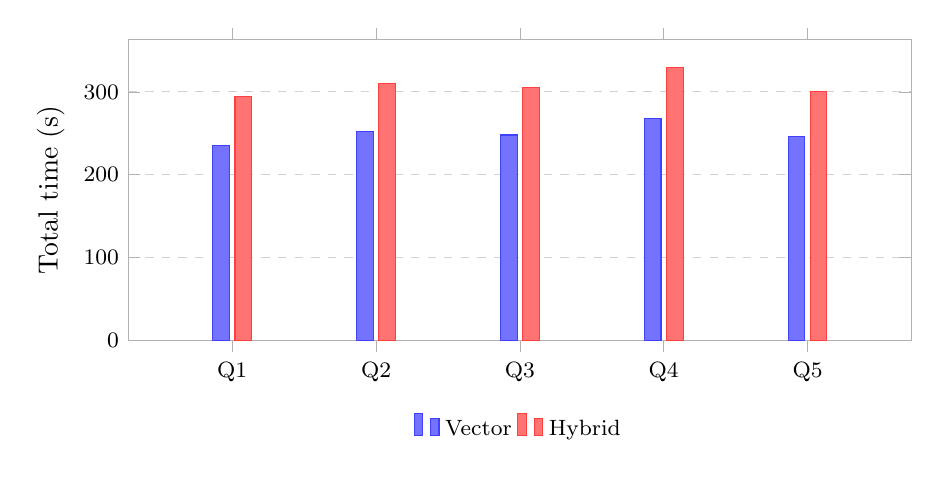
\begin{tikzpicture}
    \begin{axis}[
        ybar,
        bar width=6pt,
        width=0.95\linewidth,
        height=5.4cm,
        ylabel={Total time (s)},
        symbolic x coords={Q1,Q2,Q3,Q4,Q5},
        xtick=data,
        ymin=0,
        enlarge x limits=0.18,
        ymajorgrids=true,
        grid style={dashed,gray!35},
        axis line style={gray!60},
        tick style={gray!60},
        tick label style={font=\footnotesize},
        legend style={at={(0.5,-0.22)}, anchor=north, legend columns=2, draw=none, font=\footnotesize},
      ]
      \addplot+[fill=blue!55, draw=blue!75] coordinates {(Q1,235) (Q2,252) (Q3,248) (Q4,268) (Q5,246)};
      \addplot+[fill=red!55,  draw=red!75]  coordinates {(Q1,295) (Q2,310) (Q3,305) (Q4,330) (Q5,300)};
      \legend{Vector,Hybrid}
    \end{axis}
  \end{tikzpicture}
  \caption{Thời gian tổng theo từng câu hỏi (Q1--Q5): Vector vs Hybrid.}
  \label{fig:bench-per-q}
\end{figure}

\subsection{Ảnh hưởng chunk\_size tới thời gian}
Hình~\ref{fig:chunk-vs-time} minh hoạ xu hướng thời gian truy xuất theo các cấu hình chunking. Thực nghiệm cho thấy chunk lớn có xu hướng giảm số lượng chunks, giúp giảm chi phí retrieval, nhưng cần cân bằng để không làm mất chi tiết ngữ nghĩa.

\begin{figure}[!htbp]
  \centering
  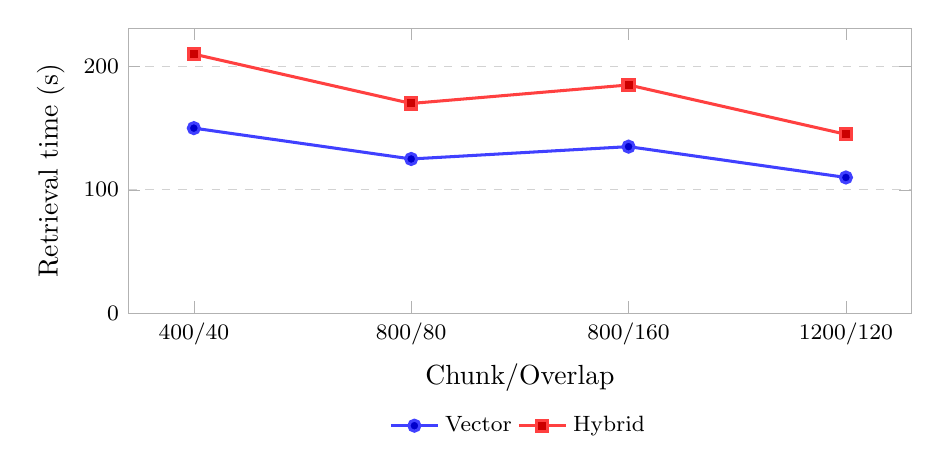
\begin{tikzpicture}
    \begin{axis}[
        width=0.95\linewidth,
        height=5.2cm,
        xlabel={Chunk/Overlap},
        ylabel={Retrieval time (s)},
        symbolic x coords={400/40,800/80,800/160,1200/120},
        xtick=data,
        ymin=0,
        ymajorgrids=true,
        grid style={dashed,gray!35},
        axis line style={gray!60},
        tick style={gray!60},
        tick label style={font=\footnotesize},
        % Đẩy legend xuống -0.32 để tránh đè lên nhãn xlabel
        legend style={at={(0.5,-0.32)}, anchor=north, legend columns=2, draw=none, font=\footnotesize},
      ]
      \addplot+[mark=*, line width=1.1pt, blue!75] coordinates {(400/40,150) (800/80,125) (800/160,135) (1200/120,110)};
      \addplot+[mark=square*, line width=1.1pt, red!75]  coordinates {(400/40,210) (800/80,170) (800/160,185) (1200/120,145)};
      \legend{Vector,Hybrid}
    \end{axis}
  \end{tikzpicture}
  \caption{Ảnh hưởng cấu hình chunking lên thời gian retrieval (minh hoạ).}
  \label{fig:chunk-vs-time}
\end{figure}

\subsection{Testing \& Test Cases}
\textbf{Công cụ:} \texttt{pytest}. Bộ kiểm thử tập trung vào các thành phần lõi để đảm bảo pipeline hoạt động ổn định và tránh lỗi hồi quy khi mở rộng tính năng.

\textbf{Các test case tiêu biểu:}
\begin{itemize}
  \item \textbf{Kiểm thử ingest multi-file:} đảm bảo sau khi ingest, mỗi chunk có metadata cần thiết (\texttt{source}, \texttt{file\_type}, \texttt{upload\_date}, \texttt{doc\_id}, \texttt{chunk\_index}).
  \item \textbf{Kiểm thử HybridRetriever:} kiểm tra cơ chế chuẩn hoá nội dung, loại trùng lặp (dedupe), và thứ tự kết quả sau bước fusion/rerank (tuỳ cấu hình).
  \item \textbf{Kiểm thử benchmark:} đảm bảo hàm benchmark trả về đầy đủ các trường thời gian (\texttt{retrieval\_time}, \texttt{generation\_time}, \texttt{total\_time}) cho cả Vector và Hybrid.
\end{itemize}

\textbf{Gợi ý lệnh chạy:}
\begin{verbatim}
pytest -q
\end{verbatim}

\subsection{Ưu điểm và Hạn chế}
\textbf{Ưu điểm:}
\begin{itemize}
  \item \textbf{Tính thực dụng cao:} hỗ trợ PDF/DOCX, multi-file và truy vết nguồn; phù hợp nhiều ngữ cảnh học tập/doanh nghiệp.
  \item \textbf{Chất lượng truy xuất linh hoạt:} Hybrid Search cải thiện khả năng bắt từ khoá chính xác trong các truy vấn chứa thuật ngữ/mã số.
  \item \textbf{Khả năng đánh giá định lượng:} benchmark giúp người dùng tự kiểm chứng hiệu quả của Vector vs Hybrid theo từng câu hỏi.
  \item \textbf{Tính bền vững:} có lưu lịch sử chat và trạng thái theo \texttt{session\_id}.
\end{itemize}

\textbf{Hạn chế:}
\begin{itemize}
  \item \textbf{Chi phí tính toán:} Hybrid (và đặc biệt Re-ranking nếu bật) có thể tăng latency so với Vector-only.
  \item \textbf{Phụ thuộc chất lượng chunking:} tham số \texttt{chunk\_size}/\texttt{chunk\_overlap} ảnh hưởng mạnh đến retrieval và câu trả lời.
  \item \textbf{Khôi phục đầy đủ index:} việc lưu/khôi phục vectorstore cần được quản lý cẩn thận để tránh sai lệch giữa DB và dữ liệu trên đĩa.
\end{itemize}

\subsection{So sánh với các giải pháp khác}
So với các hệ thống RAG cơ bản chỉ dùng Vector Search (FAISS), SmartDoc AI có các điểm khác biệt:
\begin{itemize}
  \item \textbf{Hybrid Search + benchmark:} vừa hỗ trợ tìm theo ngữ nghĩa vừa bắt từ khoá, kèm công cụ đo lường để so sánh trực tiếp.
  \item \textbf{Multi-document + metadata:} quản lý nhiều nguồn và truy vết rõ ràng theo \texttt{source}/\texttt{file\_type}/\texttt{upload\_date}.
  \item \textbf{Persistence theo session:} lịch sử hội thoại và trạng thái tài liệu được lưu bằng SQLite, giúp trải nghiệm không bị mất khi refresh.
\end{itemize}

\section{KẾT LUẬN}
\subsection{Tổng kết}
\textbf{SmartDoc AI} đã hoàn thiện pipeline RAG từ ingest tài liệu, chunking, retrieval (Vector/Hybrid), sinh câu trả lời, hiển thị nguồn, đến benchmark và lưu trạng thái phiên. Hệ thống hướng tới tính minh bạch (citation), dễ đánh giá (benchmark) và dễ mở rộng (module hoá theo chức năng).

\section{HƯỚNG PHÁT TRIỂN}
\subsection{Hướng phát triển tương lai}
\begin{itemize}
  \item \textbf{Tối ưu hiệu năng retrieval:} cache/reuse index theo \texttt{session\_id}, giảm thời gian khởi tạo lại FAISS/BM25 khi hỏi nhiều câu.
  \item \textbf{Re-ranking có kiểm soát:} cung cấp tuỳ chọn bật/tắt và cấu hình mô hình reranker theo tài nguyên máy.
  \item \textbf{Mở rộng lọc metadata \& UI:} bổ sung filter nâng cao (theo khoảng ngày, theo nhóm tài liệu) và thống nhất UI cho multi-file.
  \item \textbf{Đánh giá chất lượng (offline eval):} xây dựng bộ câu hỏi chuẩn và thước đo (precision@k, faithfulness) để đánh giá định lượng.
\end{itemize}

\section{TÀI LIỆU THAM KHẢO}
\begin{thebibliography}{20}
  \bibitem{vn-rag}
  viblo.asia, Tìm hiểu về Retrieval Augmented Generation (RAG). \url{https://viblo.asia/p/tim-hieu-ve-retrieval-augmented-generation-rag-Ny0VGRd7LPA}

  \bibitem{vectorstore}
  Langchain, Faiss integration. \url{https://docs.langchain.com/oss/python/integrations/vectorstores/faiss}

  \bibitem{ollama}
  Ollama, Local LLM runtime. \url{https://ollama.ai/}

  \bibitem{qwen}
  Alibaba Cloud, Qwen2.5 Model Suite. \url{https://github.com/QwenLM/Qwen2.5}

  \bibitem{rag-lewis2020}
  P. Lewis et al., ``Retrieval-Augmented Generation for Knowledge-Intensive NLP Tasks,'' \textit{NeurIPS}, 2020.

  \bibitem{improving-lm-retrieval}
  (Survey) ``Improving Language Models with External Knowledge Retrieval,'' arXiv preprint.

  \bibitem{dpr-karpukhin2020}
  V. Karpukhin et al., ``Dense Passage Retrieval for Open-Domain Question Answering,'' \textit{EMNLP}, 2020.

  \bibitem{realm-guu2020}
  K. Guu et al., ``REALM: Retrieval-Augmented Language Model Pre-Training,'' \textit{ICML}, 2020.

  \bibitem{atlas-izacard2022}
  G. Izacard et al., ``Atlas: Few-shot Learning with Retrieval-Augmented Language Models,'' 2022.

  \bibitem{graphrag}
  ``GraphRAG: Leveraging Knowledge Graphs for Retrieval-Augmented Generation,'' arXiv preprint.

  \bibitem{kg-aug-lm}
  ``Knowledge Graph-Augmented Language Models for Reasoning Tasks,'' arXiv preprint.

  \bibitem{structured-knowledge-rag}
  ``Integrating Structured Knowledge into Retrieval-Augmented Generation,'' arXiv preprint.

  \bibitem{graph-based-retrieval}
  ``Graph-Based Retrieval for Enhanced Text Generation,'' arXiv preprint.

  \bibitem{hybrid-graph-vector}
  ``Hybrid Graph and Vector Retrieval for Large Language Models,'' arXiv preprint.
\end{thebibliography}

\end{document}